\documentclass[conference]{IEEEtran}

\IEEEoverridecommandlockouts

\usepackage{cite}
\usepackage{amsmath,amssymb,amsfonts}
\usepackage{algorithmic}
\usepackage{graphicx}
\usepackage{textcomp}
\usepackage{xcolor}

\usepackage{booktabs} %@{}
\usepackage{pgfplots}
\pgfplotsset{compat=1.16}
\usepackage[per-mode=symbol,detect-all]{siunitx}
\usepackage{cleveref} %\Cref{} vs. \cref{}
\usepackage[protrusion=true,expansion=true]{microtype}
\usepackage{mathabx} % for \bigtimes

\def\BibTeX{{\rm B\kern-.05em{\sc i\kern-.025em b}\kern-.08em
    T\kern-.1667em\lower.7ex\hbox{E}\kern-.125emX}}

\begin{document}


\title{\LARGE \textbf{Planning Under Uncertainty with Sensor Occlusions in \\ Urban Driving Scenarios} % \\
%\thanks{Ross Alexander is supported by a Stanford Graduate Fellowship (SGF) in Science and Engineering.}
}


\author{\IEEEauthorblockN{  Ross Alexander}
\IEEEauthorblockA{\textit{  Department of Aeronautics and Astronautics} \\
\textit{                    Stanford University} \\
                            Stanford, CA 94305 \\
                            rbalexan@stanford.edu}} % or ORCID


\maketitle

\begin{abstract}
    Safe and efficient autonomous driving in urban scenarios requires a policy that is responsive to uncertainty in the environment and sensors. Partial observability of the environment due to sensor occlusions has led to conservative manually-designed driving policies that are inefficient. Collision avoidance is sequential decision-making problem under uncertainty and can be posed as a partially observable Markov decision process (POMDP), which can be solved to generate an optimal policy. We leverage the POMDP formulation to generate approximately optimal collision avoidance policies and evaluate the safety and efficiency of the resulting driving behaviors. We find that the policies outperform baseline policies and are generally highly-performant and robust to uncertainty in the environment and sensors.
\end{abstract}

% \begin{IEEEkeywords}
% component, formatting, style, styling, insert
% \end{IEEEkeywords}

\section{Introduction}
\label{sec:introduction}

% Overview of topic sentences
Autonomous driving in urban scenarios requires navigating safely and efficiently in light of significant uncertainty presented by occlusions. In dense urban settings, buildings, signs, cars, and other physical obstacles frequently occlude other road users from the field of view of the sensors. Planning in these occluded scenarios requires judicious safety thresholds in order to ensure collision-free driving. In this paper, we focus on developing safe and efficient policies for collision avoidance while passing a crosswalk with pedestrians emerging from an occluded region.

% What is the problem?                     
We consider the occluded crosswalk scenario depicted in \cref{fig:occluded_crosswalk_scenario}. The scenario consists of an autonomous vehicle driving along a roadway and a pedestrian crossing the roadway at a crosswalk. The ego vehicle's sensors are occluded by a static obstacle that prevents the pedestrian from being observed. 

\begin{figure}[htbp]
    \centerline{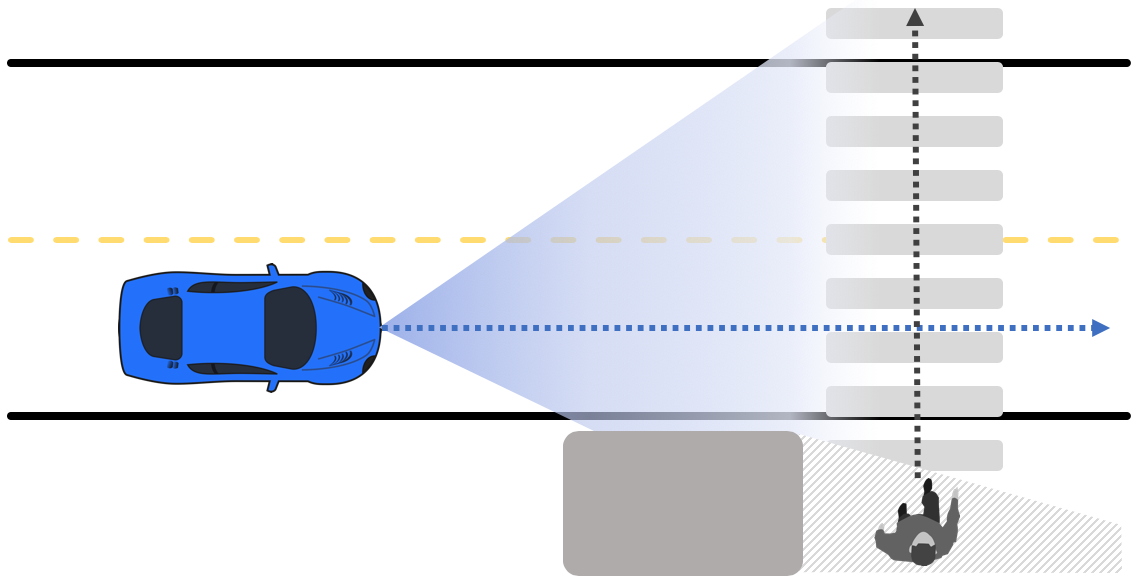
\includegraphics[width=0.95\linewidth]{doc/main/occluded_crosswalk_scenario.png}}
    \caption{The occluded crosswalk scenario. The ego vehicle (in blue) is driving along the roadway and the pedestrian (in gray) is crossing the crosswalk. The static obstacle occludes the ego vehicle's sensors and prevents observation of the pedestrian.}
    \label{fig:occluded_crosswalk_scenario}
\end{figure}

% Why is it interesting and important?
% Why is it hard? Why do naive approaches fail?
Urban driving scenarios are often heavily occluded, which presents significant challenges in achieving fully autonomous driving. Occlusions in urban scenarios can arise as a result of \textit{static obstacles}, such as buildings, signs, and parked cars, but occlusions can also arise as a result of \textit{dynamic obstacles}, such as moving pedestrians and moving cars. Above all, the autonomous vehicle must navigate safely and avoid collision with pedestrians. However, the autonomous vehicle must also navigate efficiently and cannot be paralyzed by the significant uncertainty of pedestrians potentially occupying an occluded region. Even when a pedestrian is not occluded, sensor uncertainty due to noise often precludes a full understanding of a pedestrian's pose. The trade-off between safety and efficiency is captured strongly by the occluded crosswalk scenario. Optimizing this trade-off and generating a driving policy that is safe and robust to uncertainty in the environment and sensors is a critical step in urban autonomous driving.

% \textbf{Why hasn't it been solved before? (Or, what's wrong with previous proposed solutions? How does mine differ?)}
% other planning frameworks exist - topic sentence
Several planning frameworks already exist to ensure collision-free paths when passing occluded regions. If dynamic objects emerging from occluded regions have a bounded velocity, the autonomous vehicle can follow a maximal velocity profile along its original planned path that ensures a collision-free trajectory \cite{Alami2002OnPlans}. A variety of approaches use autonomous emergency braking (AEB) systems to perform collision avoidance maneuvers. The time-to-collision (TTC) metric and several extensions of the TTC metric have shown to be reliable safety measures not only for vehicle collision avoidance \cite{Minderhoud2001ExtendedAssessment}, but also for pedestrian collision avoidance, provided we can infer pedestrian intentions and predict the resulting movements \cite{Volz2019InferringCrosswalks}. While these planning frameworks are effective at ensuring essentially collision-free driving, they suffer from uncertainty in the environment and sensors that can create inefficient control policies likely to initiate unnecessary severe rapid braking.

% expanding to multiple road users
%-- the so-called "full-stop."
% what do we do in this work

% Modeling as a POMDP - topic sentence
In order to develop driving policies robust to uncertainty in the environment and sensors, others have chosen to model the collision avoidance problem as a partially observable Markov decision process (POMDP). 

A scalable approach to avoiding multiple occluded pedestrians was achieved through utility fusion \cite{Bouton2018ScalableDriving}. The multiple road user collision avoidance problem was decomposed into single road user collision avoidance sub-problems enabling solution of the problem that scales linearly with the number of road users considered. The set of single road user optimal belief action utilities were synthesized to generate an approximation to the optimal belief action utility for all road users using a fusion function. The authors consider both sum and minimum fusion functions and find the minimum fusion function generates a more conservative policy. Others have expanded on the success of the multiple occluded road user longitudinal-control policy and developed in-lane coupled longitudinal- and lateral-control policies that maintain safety and improve scenario crossing speeds \cite{Schratter2019PedestrianOcclusions}.

with a flow of pedestrians using offline  \cite{Thornton2019TowardValues,Bouton2018ScalableDriving}. and in-lane coupled longitudinal- and lateral-control policies that 

Moreover, planning in occluded scenarios requires reasoning about the occluded region and the state of any potential traffic participant in the region. This partial observability presented by occlusions leads traditional algorithms to fail to predict hidden participants and typically results in significantly higher collision rates in urban collision scenarios. We also need to do it in simulation. We also need to find corner cases (adaptive stress testing). Discretization v continuous and size of state space, observation. Requires complex generative model or detailed explicit transition model. Consider the simplest case in order to understand approaches that work well in broad strokes for solving these planning under uncertainty problems.

%\textbf{What are the key components of my approach and results? Also include any specific limitations.}
This paper recreates results from 

In this paper, we consider the problem of avoiding collisions with pedestrians crossing behind an occluded region on the side of the road. 

% Summary of the major contributions in bullet form, mentioning in which sections they can be found. This material doubles as an outline of the rest of the paper, saving space and eliminating redundancy.
We discuss related work in \cref{sec:related-work} and describe the partially-observable Markov decision process (POMDP) and solution techniques for generating an approximately optimal policy in \cref{sec:background}. \Cref{sec:proposed-approach} discusses how the collision avoidance problem can be posed as a POMDP and the solution approaches we take in obtaining an approximately optimal policy. \cref{sec:experiments,sec:results} cover the experimental setup, analysis of the safety and efficiency criteria, and discussion of the resulting driving policies. Finally, we present our conclusions in \cref{sec:conclusion} and provide some areas for further research in \cref{sec:future-work}.


\section{Related Work}
\label{sec:related-work}

\section{Background}
\label{sec:background}

A principled and general framework for planning under uncertainty is the partially-observable Markov decision process (POMDP). A POMDP is typically defined by the tuple $\langle \mathcal{S},\mathcal{A}, \mathcal{O}, T, R, O, \gamma \rangle$, where $\mathcal{S}$ is the state space, $\mathcal{A}$ is the action space, $\mathcal{O}$ is the observation space, $T$ is the transition model, $R$ is the reward model, $O$ is the observation model, and $\gamma$ is the discount factor. An agent in state $s \in \mathcal{S}$, takes action $a \in \mathcal{A}$, and transitions to a state $s' \in \mathcal{S}$ with probability $T(s, a, s') = \textnormal{Pr}(s' \mid s, a)$. Then, the agent observes $o \in \mathcal{O}$ with probability $O(o, s',a) = \textnormal{Pr}(o\mid s', a)$ and receives a real-valued reward $R(s, a)$. 

% belief representation, % belief update % belief is a c
In a POMDP, the state of the environment may not be fully observable, so the agent maintains a belief $b$ about the underlying state. The belief state is a categorical probability distribution over the state space that lies in the standard $|\mathcal{S}|-1$ simplex $\Delta^{|\mathcal{S}|-1}$, so that $b(s): \mathcal{S} \rightarrow [0,1]^{|\mathcal{S}|}$ subject to the constraint $\sum_{s\in \mathcal{S}} b(s) = 1$. The belief $b$ is updated after taking action $a$ and observing $o$ using the Bayesian belief update:
\begin{equation}
    b'(s')~\propto~O(o \mid s', a) \sum_{s \in S} T(s' \mid s, a) b(s)
\end{equation}

% intractability and citation
% online and offline methods
% QMDP, SARSOP, and other solvers + brief descriptions
The solution to a POMDP is an optimal policy $\pi^*$ that maps beliefs to actions. Following the optimal policy from any initial state maximizes the expected discounted sum of future rewards. % value function U*(b,a)

\section{Proposed Approach}
\label{sec:proposed-approach}

\subsection{POMDP Model}

In this approach, the state of each traffic participant $p$ in the set of traffic participants $\mathcal{P}$ is defined by a tuple $(s_p, v_p)$. In the occluded crosswalk problem, we track the ego vehicle's position along the roadway $s_{ego}$ and the ego vehicle's velocity $v_{ego}$. Similarly, we track the pedestrian's position along the crosswalk $s_{ped}$ and the pedestrian's velocity $v_{ped}$. The state space for the occluded crosswalk problem is represent as $\mathcal{S} = (s_{ego}, v_{ego}) \times (s_{ped}, v_{ped})$. It is straightforward to extend the model to more complex urban driving scenarios with additional traffic participants where the state space has the representation $\mathcal{S} = (s_{ego}, v_{ego}) \bigtimes_{p\in\mathcal{P}}(s_p, v_p)$

\subsubsection{State space} For the occluded crosswalk scenario, we track the poses of the ego vehicle and the pedestrian in the Fren\'et frame. The ego vehicle pose consists of the position along the lane and the velocity in the lane $(s_{ego}, v_{ego})$. Similarly for the pedestrian, the pose consists of the position along the crosswalk and the velocity in the crosswalk $(s_{ped}, v_{ped})$. We assume in general that the crosswalk is orthogonal to the roadway.

\subsubsection{Action space} The ego vehicle's actions consist of the set of accelerations $\mathcal{A} = \{-2~\si{\meter\per\square\second}, -1~\si{\meter\per\square\second}, 0~\si{\meter\per\square\second}, 1~\si{\meter\per\square\second}\}$. The accelerations are designed to map to standard strategic maneuvers -- rapid deceleration, deceleration, continuation, and acceleration, respectively.

\subsubsection{Observation space} The observation space is similar to the state space. The ego vehicle's pose is assumed to be perfectly observable. If the pedestrian is occluded, the pedestrian's pose is unobserved ($p_{absent}$). If the pedestrian is not occluded, the pedestrian's pose is partially observable with the position and velocity following Gaussian distributions centered on the true value. \footnote{with what params} $o_{s_{ped}} \sim \mathcal{N}(o_{s_{ped}} \mid \mu_s, \sigma_s)$ and $o_{v_{ped}} \sim \mathcal{N}(o_{v_{ped}} \mid \mu_v, \sigma_v)$.

\subsubsection{Transition model} The evolution of the ego vehicle is given by a simple constant acceleration model that follows:
\begin{align}
    a_t &= a_{ego} \nonumber \\
    v_t &= v_{t-1} + a_t \Delta t \\
    s_t &= s_{t-1} + v_t \Delta t + \tfrac{1}{2} a_t \Delta t^2 \nonumber
\end{align}
The pedestrian evolves using a simple constant velocity model where the velocity at the following time step is sampled according to a uniform distribution over a set of velocities $V = \{-1~\si{\meter\per\second}, 0~\si{\meter\per\second}, 1~\si{\meter\per\second}\}$ $v \sim \mathcal{U}(v \mid v \in V)$
\begin{align}
    v_t &= v \nonumber \\
    s_t &= s_{t-1} + v_t \Delta t 
\end{align}

\subsubsection{Reward model} Rewards are discounted using a discount factor $\gamma = 0.95$\footnote{verify this}, which encourages the agent to seek immediate rewards over future rewards.  



\subsection{POMDP Solvers}

We use the following two offline methods to generate approximately optimal policies

\subsubsection{QMDP}
QMDP solve the POMDP by assuming full observability at the following time step. \cite{Littman1995LearningUp}

full observability at the next time step

\subsubsection{SARSOP}
Successive Approximation of the Reachable Space under Optimal Policies 
\cite{Kurniawati2009SARSOP:Spaces}

 % number of total states after discretization

\section{Experiments}
\label{sec:experiments}

Experiments

\section{Results}
\label{sec:results}


Results and Discussion

\section{Conclusion}
\label{sec:conclusion}


%\textbf{In general a short summarizing paragraph will do, and under no circumstances should the paragraph simply repeat material from the Abstract or Introduction. In some cases it's possible to now make the original claims more concrete, e.g., by referring to quantitative performance results.}

\section{Future Work}
\label{sec:future-work}


\bibliographystyle{IEEEtran}
\bibliography{main}

\end{document}

%\begin{table}[htbp]
%    \caption{Table Type Styles}
%    \begin{center}
%        \begin{tabular}{|c|c|c|c|}
%            \hline
%            \textbf{Table}&\multicolumn{3}{|c|}{\textbf{Table Column Head}} \\
%            \cline{2-4} 
%            \textbf{Head} & \textbf{\textit{Table column subhead}}& \textbf{\textit{Subhead}}& \textbf{\textit{Subhead}} \\
%            \hline
%            copy& More table copy$^{\mathrm{a}}$& &  \\
%            \hline
%            \multicolumn{4}{l}{$^{\mathrm{a}}$Sample of a Table footnote.}
%        \end{tabular}
%        \label{tab1}
%    \end{center}
%\end{table}